\section{Software qualities and architectures}

Numerous software qualities are directly shaped by architectural decisions, necessitating metrics to quantify these qualities and methodologies to analyze the quantitative impact of architectural choices on them.

\subsection*{Availability}
Continuous availability of a service is imperative to ensure minimal downtime and rapid service recovery.
The service's availability depends on several factors, including:
\begin{itemize}
    \item Complexity of IT infrastructure architecture.
    \item Reliability of individual components.
    \item Ability to respond quickly and effectively to faults.
    \item Quality of the maintenance by support organizations and suppliers.
    \item Quality and scope of the operational management processes.
\end{itemize}

\begin{definition}
    The \emph{time of occurrence} is the time at which the user becomes aware of the failure. 

    The \emph{detection time} is the time at which operators become aware of the failure. 

    The \emph{response time} is the time required by operators to diagnose the issue and respond to users. 

    The \emph{repair time} is the time required to fix the service or components that caused the failure. 

    The \emph{recovery time} is the time required to restore the system. 

    The \emph{mean time to repair} (MTTR) is the average time between the occurrence of a failure and service recovery, also known as the downtime. 

    The \emph{mean time to failures} (MTTF) is the average time between the recovery from one failure and the occurrence of the next failure, also known as uptime.

    The \emph{mean time between failures} (MTBF) is the average time between the occurrences of two consecutive failures. 
\end{definition}
\begin{figure}[H]
    \centering
    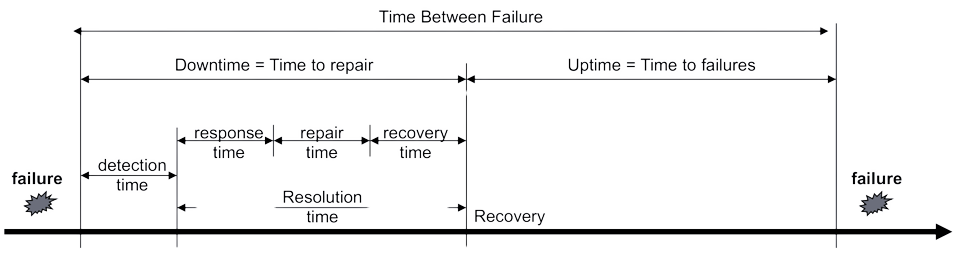
\includegraphics[width=0.75\linewidth]{images/fail.png}
\end{figure}
\begin{definition}
    The \emph{availability metric} is a probability that a component is working properly at time $t$, defined as: 
    \[A=\dfrac{\textnormal{MTTF}}{\textnormal{MTTF}+\textnormal{MTTR}}\]
\end{definition}
Availability is typically specified in nine notation (indicating the number of consecutive nines in the percentage). 

Availability is calculated by modeling the system as an interconnection of elements in series and parallel:
\begin{itemize}
    \item Elements operating in series. 
        If an element in the series fails, it results in the failure of the entire combination.
        \[A_{\textnormal{series}}=\prod_{i=1}^n A_i\]
        A chain's strength is determined by its weakest link.
    \item Elements operating in parallel. 
        In this scenario, the failure of one element prompts the other elements to assume the operations of the failed component.
        \[A_{\textnormal{parallel}}=1-\prod_{i=1}^n (1-A_i)\]
        Critical systems are often designed with redundant components to enhance reliability and availability.
\end{itemize}

The main techniques employed to enhance availability include replication, forward error recovery, and circuit breakers.

Replication can be done in multiple ways: 
\begin{itemize}
    \item Hot spare: one leading server with another always ready to take over.
    \item Warm spare: leading server periodically updates another; if the leading one fails, some time may be needed to fully update the backup.
    \item Cold spare: backup server is dormant and started/updated only when needed.
    \item Triple modular redundancy: multiple active servers, and the produced result is based on the majority.
\end{itemize}

For the forward error recovery we have that in the failure state, a recovery mechanism moves the component to the degraded state.
In the degraded state, the component continues to be available even if not fully functional.